\chapter{Style-based Tone mapping}
\label{chp:b5}

HDR image similarity has many applications, and one of these applications on tone mapping is presented in this chapter. The tone mapping operator that is depicted in the following sections named as style-based tone mapping, consists of a methodology that employs image similarity to tone map HDR images consistently according to a style without manual parameter adjustments. In this chapter, first the problem definition and related work is given followed by the details of the method and the obtained tone mapping results. Lastly, the improvements made to the initial method using the findings of the user experiment is presented.

\section{Problem Definition}

Tone mapping operators aim to reduce the dynamic range of an HDR image to display it on an low dynamic range display devices. The existence of numerous tone mapping operators that are available paved the way for many studies that are conducted for selecting the best one~\cite{parraga2018tone}. However, tone mapping can be conducted for different purposes, and rendering the resulting images to follow a consistent style can be one of them. For example, in a movie production process, making all frames consistently tone mapped, regardless of the content of the frames, can be a desired operation to impart a certain look and feel to the viewers. Although obtaining different renderings from tone mapping operators is partly achievable by using different tone mapping parameters, some tone mapping operators have none~\cite{Dura02} or few parameters~\cite{Fatt02} while others~\cite{Photomatix2010} have too many. Besides, even though one set of parameters are found for a certain image to depict a certain style of rendering, the same set of parameters would not yield with the same look when applied to other images. %that has different characteristics.

In this chapter, style based tone mapping operator that aims to consistently tone map different HDR images with the defined style is proposed. Figure \ref{fig:styles} shows different styles for the same images created by an artist. The application depicted in this thesis approaches the problem of defining a style by presenting the user an HDR image and with the help of the tool developed, ask the user to change the parameters until the image matches the desired look. By repeating this process for a small set of calibration images, we aim to \emph{learn} the style. Applying the learned style from calibration images to the previously unseen images is essentially a visual image similarity problem.

\begin{figure}
\begin{center}
\includegraphics[width=\textwidth]{figures/chapter5/styles.png}
\caption{Different artists may prefer different tone reproductions of the same HDR image. The same artist may also choose to produce different styles based on the situational/contextual considerations. The images reproduced by a professional artist using a different tool (top half) are replicated using our operator (bottom half). Presented algorithm can also learn the styles of an artist and produce results consistent with them.}
\label{fig:styles}
\end{center}
\end{figure}
%First, the problem of relating the input HDR image and the calibration images are solved with a method that has been commonly used for LDR images in the earlier work and then two different but related methods that uses the findings from the user experiment of visual similarity for HDR images discussed in Chapter \ref{chp:b3} and Chapter \ref{chp:b4} are employed.
%To summarize, the primary difference of the current method from the earlier work is its ability to learn about the various tone mapping styles that may be desired by an artist from a small set of calibration images. These styles can then be applied when tone mapping a new HDR image. Our algorithm is the first of its kind that gives the ability to batch process a large number of HDR images with respect to different styles.

\section{Related Work}
Image reproduction is ultimately a subjective process where photographers and artists of all persuasions are free to reflect their own interpretation into the final rendering. For any task of reproduction, there is generally a vast range of choices from literal or realistic reproduction to those that significantly depart from reality. Since the early days of photography, many tools and systems have been developed to enable artists express their creativity~\cite{Adams80,Adams81,Adams83,White84}.

Tone mapping, in the context of HDR imaging, is no different in creative expression than the art of photography. There is essentially an infinite amount of choices that an artist can make when tone mapping an HDR image for display purposes (Figure~\ref{fig:styles}). Perhaps, this is underscored by the large number of TMOs that have so far been developed that produce different outputs from the same HDR image~\cite{Rein2010}.

Most TMOs fail to provide sufficient freedom to artists to express their creativity and rather focus on visibility or photographic look. However, there are a few TMOs that are designed to enable artistic freedom such as the stroke-based interface that was proposed by Lischinski et al.~\cite{Lischinski2006}. This algorithm allows the user to select image regions using brush strokes and set different tone mapping parameters for each region. These parameters are then extrapolated to the entire image using an edge-preserving energy minimization method. Paris et al.~\cite{paris2011local} gives users the possibility of enhancing details or edge-preserving smoothing while tone mapping. This method first applies detail modifying local Laplacian filters on the log intensity of the image and then map the intensities to displayable range by scaling. Aubry et al.~\cite{aubry2014fast} offers a fast implementation of local Laplacian filters and also demonstrates how this filter can be used for photographic style transfer. Given a model image, this iterative method uses local Laplacian filters for gradient histogram matching for local contrast modification and intensity histogram matching for global contrast modification. Tone mapping is achieved through the intensity matching since the method matches the same dynamic range of the model image.

Another algorithm that allows a wide range of possibilities during tone mapping is the generic TMO~\cite{Mantiuk08a}. This operator hinges on the idea that although a large number of TMOs exist, the majority of them can be modeled using a generic tone curve followed by local modifications. The authors have demonstrated that by using a small set of parameters, a skilled artist can match the output of any TMO with the generic TMO. Although these algorithms offer expressive freedom to the artist, they have no notion of \emph{learning} the artist's preference. In fact, it has been shown by the authors that the same set of parameters can give rise to vastly different outputs for different images~\cite{Mantiuk08a}. As such, using these operators to automatically tone map a large number of images is impractical. 

There are several LDR retouching studies that are similar to the proposed style based tone mapping operator in the sense of enhancing images by using a set of training images ~\cite{kang2010personalization, bychkovsky2011learning} or by automatic exposure correction~\cite{yuan2012automatic} or artistic enhancement~\cite{son2014art}. However, these studies do not focus on HDR image tone mapping.

Recently, deep neural networks are also used for learning image adjustment parameters. Some of these studies uses a training set of high quality images and learns the enhancement parameters in an unsupervised manner~\cite{park2018distort, chen2018deep,ignatov2018wespe}. These methods aim to enhance the general quality of the given image instead of applying a specific style. Yan et al.~\cite{yan2016automatic} on the other hand, proposes to learn a computational model of a style from image pairs, an untouched image and a stylized version. Their method incorporates high level semantic information of the pixels as well as local and global features of the image. Another study with a similar goal, Hu et al.~\cite{hu2018exposure} uses unpaired data, a set of stylized images, for learning an operation sequence that will style an input image when applied. The benefit of learning modification steps is it makes the style explainable, which most of the deep learning based image enhancements methods lack. While these methods aim to learn predefined style, Lee et al.~\cite{lee2016automatic} uses deep learning based semantic search to find similar images from a large collection and applies the styles of these images to the given image, by using a transfer function for color and luminance statistics, which brings the benefit of automatically selecting candidate styles. Similar to the previous LDR retouching studies, these methods also do not aim to tone map HDR images.

Besides of these studies that learns image adjustment parameters using deep neural networks, initiated with the study of Gatsy et. al~\cite{gatys2016image}, deep neural networks are also used for style transfer between images. The algorithm introduced in~\cite{gatys2016image} separates and recombines the content and style of images using different layers of pretrained VGG19 network. After Gatsy et. al~\cite{gatys2016image}, neural style transfer gained popularity and many studies focused on improving this method. Gatsy et. al~\cite{gatys2017controlling} introduced control methods such as color, scale and spatial control, Gupta et. al~\cite{gupta2017characterizing} improves stability, Liu and Lai~\cite{liu2017depth} added depth awareness, Huang and Belongie~\cite{huang2017arbitrary} made the neural style transfer more practical with a faster method and flexible user controls.

In Figure~\ref{fig:neural_style_transfer}, the neural style transfer method~\cite{gatys2016image} is applied to the tone mapped HDR images. All images are taken from Fairchild's HDR dataset~\cite{fairchild2007hdr}. Content images are tone mapped with Reinhard et. al~\cite{reinhard2002photographic}, and style images are tone mapped manually with the method that is described in Section~\ref{sec:calibration} according to the \emph{candy} style shown in Figure~\ref{fig:styles}. For neural style transfer method, \emph{conv5\_2} is used as content layer, while \emph{conv1\_1} is used as style layer, content weight $\alpha = 0.1$ and style weight $\beta = 10^4$. Style transfer results are given in Figure~\ref{fig:neuro_style_result_1} and Figure~\ref{fig:neuro_style_result_2}. As shown in the resulting images and stated in the original study~\cite{gatys2016image}, it is not possible to completely separate the content and style of the images, and this method performs pleasing when artistic images like paintings are used as style images and not so well when photographs are given as style images. It is possible to see this effect in the resulting images, the edges and some objects are deformed, it is not possible to read the writings in the images, and the images looks more like a painting although given style images do not have this property.

\afterpage{
\begin{landscape}
\begin{figure}
\centering
\begin{subfigure}[b]{0.41\textwidth}
    \centering
    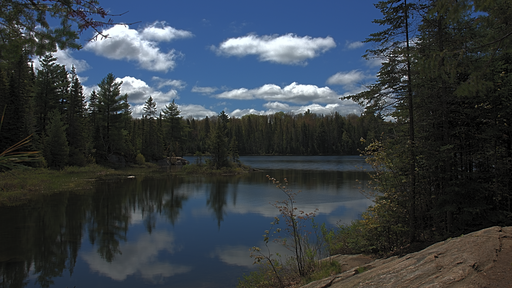
\includegraphics[width=\textwidth]{figures/neuro_style_transfer/PeckLake.hdr_candy.png}
    \caption{Style image}
\end{subfigure}\hfill
\begin{subfigure}[b]{0.41\textwidth}
    \centering
    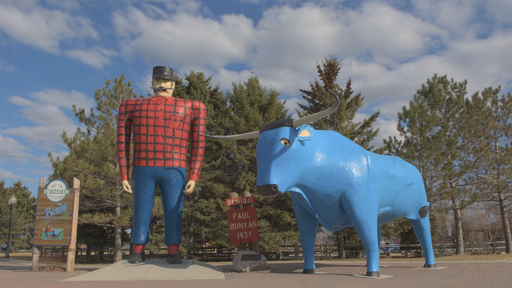
\includegraphics[width=\textwidth]{figures/neuro_style_transfer/PaulBunyan_reinhard02.png}
    \caption{Target image}
\end{subfigure}\hfill
\begin{subfigure}[b]{0.41\textwidth}
    \centering
    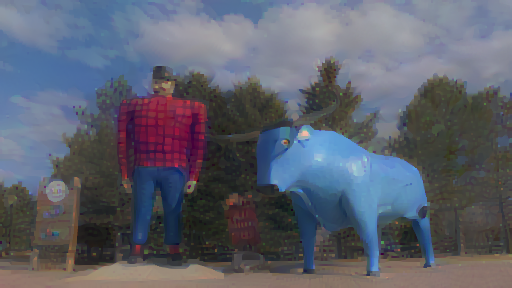
\includegraphics[width=\textwidth]{figures/neuro_style_transfer/PaulBunyan_0.1_10000.0_candy.png}
    \caption{Gatsy et. al~\cite{gatys2016image}}
    \label{fig:neuro_style_result_1}
\end{subfigure}\hfill
\begin{subfigure}[b]{0.41\textwidth}
    \centering
    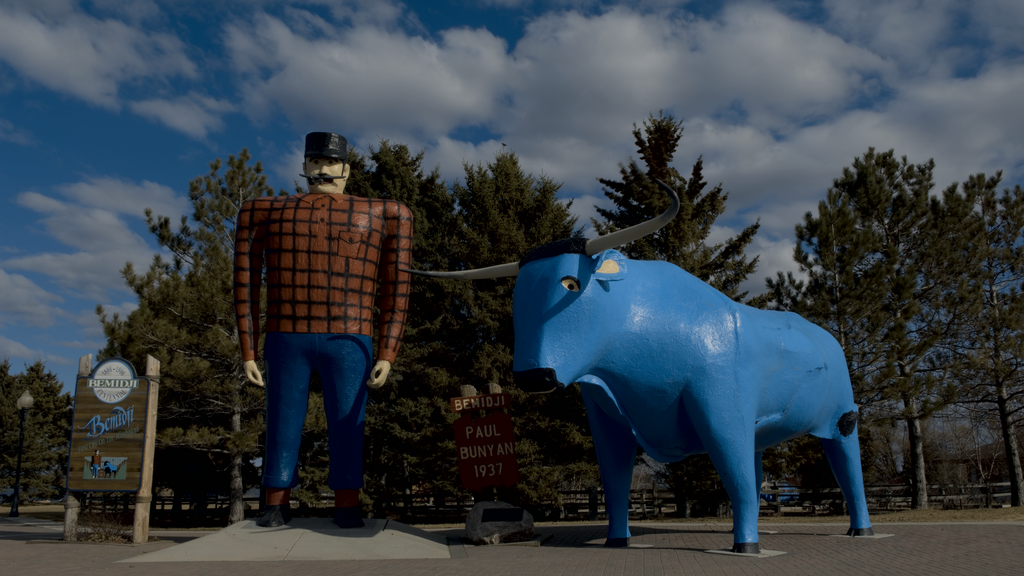
\includegraphics[width=\textwidth]{figures/reinhard_color_transfer/PaulBunyan_PeckLake_candy.png}
    \caption{Reinhard et. al~\cite{reinhard2001color}}
    \label{fig:reinhard_color_result_1}
\end{subfigure}\hfill\\ 
\begin{subfigure}[b]{0.41\textwidth}
    \centering
    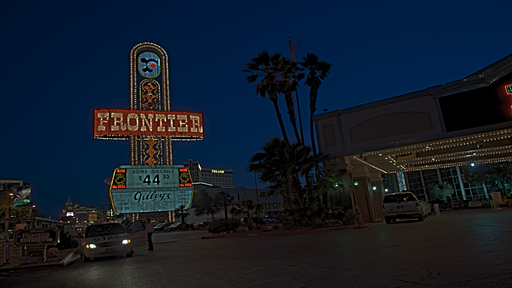
\includegraphics[width=\textwidth]{figures/neuro_style_transfer/Frontier.hdr_candy_scaled.png}
    \caption{Style image}
\end{subfigure}\hfill
\begin{subfigure}[b]{0.41\textwidth}
    \centering
    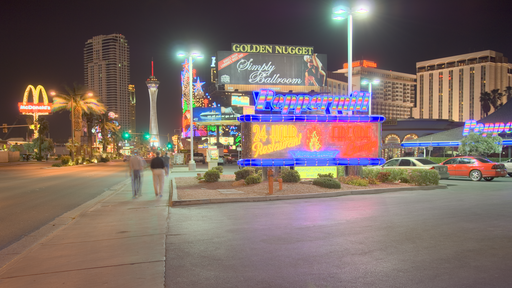
\includegraphics[width=\textwidth]{figures/neuro_style_transfer/Peppermill_reinhard02.png}
    \caption{Target image}
\end{subfigure}\hfill
\begin{subfigure}[b]{0.41\textwidth}
    \centering
    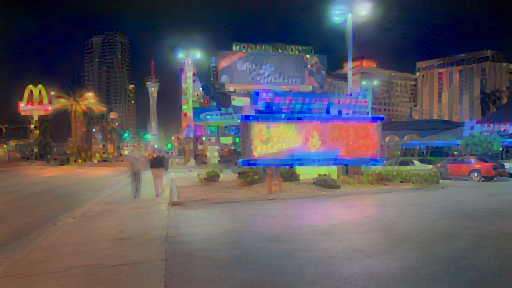
\includegraphics[width=\textwidth]{figures/neuro_style_transfer/Peppermill_0.1_10000.0_candy.png}
    \caption{Gatsy et. al~\cite{gatys2016image}}
    \label{fig:neuro_style_result_2}
\end{subfigure}\hfill
\begin{subfigure}[b]{0.41\textwidth}
    \centering
    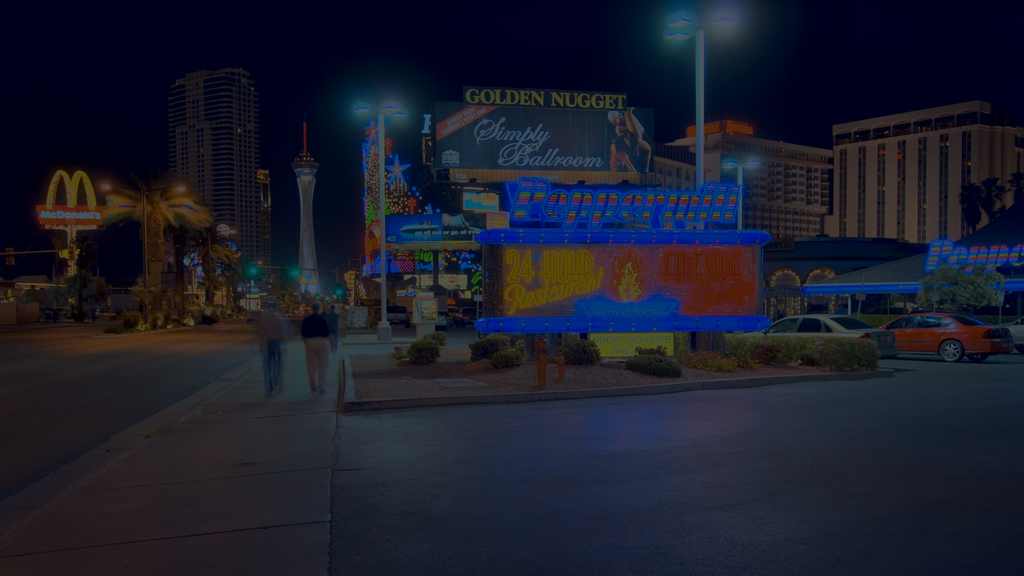
\includegraphics[width=\textwidth]{figures/reinhard_color_transfer/Peppermill_Frontier_candy.png}
    \caption{Reinhard et. al~\cite{reinhard2001color}}
    \label{fig:reinhard_color_result_2}
\end{subfigure}\hfill
\caption{Style transfer results of Gatsy et. al~\cite{gatys2016image} and color transfer results of Reinhard et. al~\cite{reinhard2001color}.}
\label{fig:neural_style_transfer}
\end{figure}
\end{landscape}}

This drawback of neural style transfer is addressed by Luan et. al~\cite{luan2017deep} by preventing spatial distortions and allowing transformations only in color space. Also by including semantic segmentation, the style transfer between unrelated contents are prevented. While this method produces very pleasing results for style transfer between images depicting similar scenes but different color palette or time of the day, it is not fully free of distortions such as creating patterns on uniformly colored objects or changing the illumination on an object in an unnatural way. Also the success of the method depends on the underlying segmentation method. On the other hand, color transfer method of Reinhard et. al~\cite{reinhard2001color} is a global method that uses simple image statistics to transfer color from one image to another. In Figure~\ref{fig:reinhard_color_result_1} and Figure~\ref{fig:reinhard_color_result_2}, the result of this method on tone mapped HDR images are given. In both results, overall brightness and contrast decreased, although both style images have bright regions similar to the content images, i.e. clouds, small light sources. 

In summary, style based tone mapping differs from the previous methods by means of learning different tone mapping styles from a small set of tone mapped calibration images. Then, new HDR images, which may be created from vastly different scenes, can be tone mapped according to these learnt styles. In this sense, style based tone mapping is the first method that allows to batch process a set of HDR images consistently according to the created style.

\section{Method}
Style based tone mapping ~\cite{akyuz2013style} consists of two consecutive phases, namely \emph{calibration} and \emph{operation}. Calibration is the phase where the user defines a style and by manually adjusting the provided parameters tone maps a small set of images until the tone mapped image depicts the newly defined style. The next phase, operation is the phase that the user given HDR image is tone mapped automatically with the selected predefined style in the calibration phase by estimating the tone mapping parameters from the calibration image tone mapping parameters. Figure \ref{fig:calibration_operation} shows the style based tone mapping algorithm steps and these steps are explained in detail in the following sections.

\begin{figure}
\begin{center}
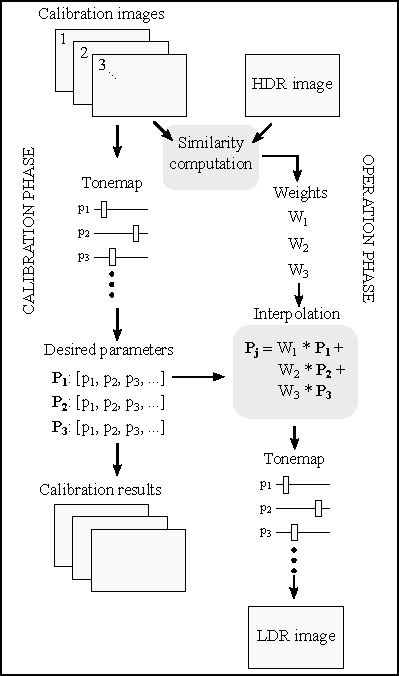
\includegraphics[width=0.65\textwidth]{figures/chapter5/algorithm.pdf}
\caption{Style based tone mapping is comprised of a calibration and operation phase. The artist tone maps several images during calibration which results in a set of parameters. During operation, these parameters are interpolated based on image similarity to find the tone mapping parameters for the given image.}
\label{fig:calibration_operation}
\end{center}
\end{figure}

\subsection{Calibration}
\label{sec:calibration}
In the calibration phase, first the user is asked to pick a name for the new style to be created, and then the user is asked to tone map a fixed set of calibration images. Assigning a name to the style would be helpful for the user to stay consistent with the style while tone mapping the calibration images. In addition, once the style is created and saved, this will allow the user to have many predefined styles in preset library and reuse them. 

Calibration images should be representative enough for different environments that has different characteristics and at the same time distinctive from each other as much as possible to keep the number of the calibration images low. The number of calibration images directly affects the time spent in the calibration phase, so although more calibration images would represent different environments better, in order not to overwhelm the user, the number of calibration images is chosen in a way that the user can finish the calibration phase in a reasonable time.

Calibration images are selected in a semi automatic way. First, all images are taken from Fairchild's HDR image dataset~\cite{fairchild2007hdr} and then converted a feature space and using k-means algorithm each image in the dataset assigned to a cluster, which resulted in six clusters given in Appendix~\ref{app:clusters}. After clusters are obtained, one calibration image is hand-selected from each cluster, yielding six calibration images in total, which are shown in Figure \ref{fig:calibration_images}.

\begin{figure}
\begin{center}
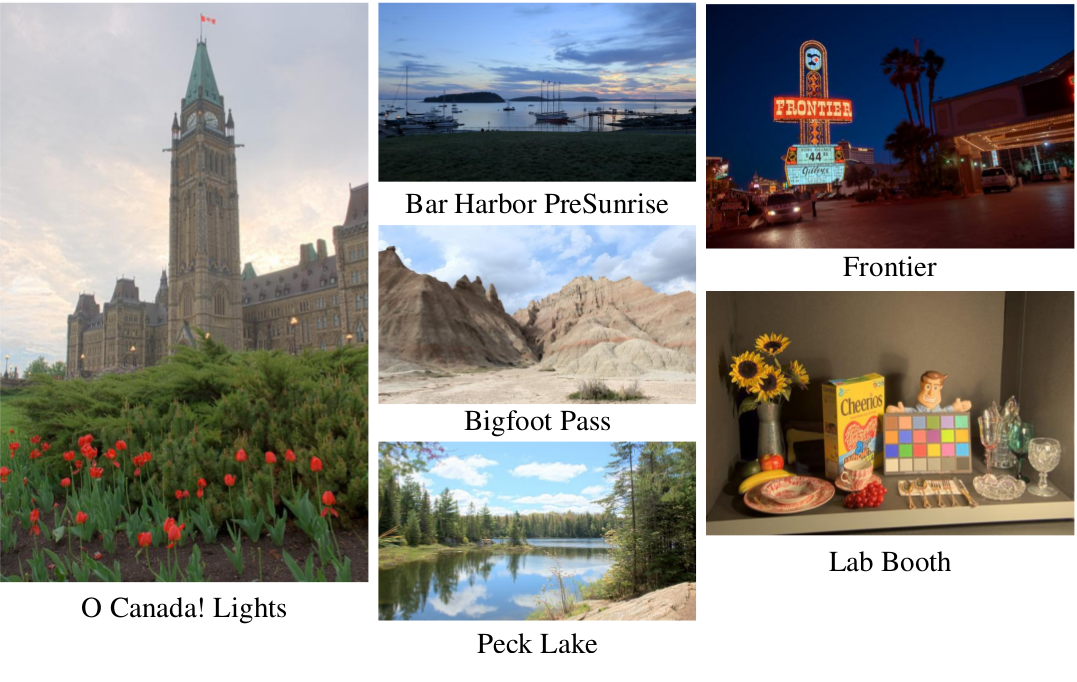
\includegraphics[width=\textwidth]{figures/chapter5/temp_calibration_images.png}
\caption{Calibration images
%paper
}
\label{fig:calibration_images}
\end{center}
\end{figure}

The calibration phase starts with naming the style, and then the user is presented with the tone mapping interface. With using this interface the user is required to tone map the calibration images one after another with the desired style. The manual tone mapping procedure is basically adjusting tone mapping parameters given in Table \ref{tab:tonemap_parameters} with the provided sliders.

\begin{table}
\caption{Tone mapping parameters for style-based tone mapping}
\label{tab:tonemap_parameters}
\centering
\begin{tabular}{|c|c|}
\hline 
Brightness ($b$) & Prct. mapped to half-max intensity \\
Contrast ($c$) & Slope of the tone curve at $b$ \\
Black point ($bp$) & Prct. clamped to min intensity \\
White point ($wp$) & Prct. clamped to max intensity \\
Color saturation ($c$) & Saturation control exponent \\
\hline
Small detail strength ($\lambda_s$) & UM factor for small details \\
Medium detail strength ($\lambda_m$) & UM factor for medium details \\
Large detail strength ($\lambda_l$) & UM factor for large details \\
\hline
\end{tabular}
\end{table}

The tone mapping operator is a modified version of Generic TMO~\cite{mantiuk2008modeling}. Generic TMO is able to model many existing tone mapping operators, both local and global with a tone curve followed by a spatial modulation function. It is noted in~\cite{mantiuk2008modeling} that same set of parameters yields very different results for different images. Style based tone mapping uses Generic TMO with the following modifications.

The tone mapping parameters of Generic TMO are replaced with their percentile counterparts in order to make the algorithm less image dependent and make it easier for user to have an understanding about the parameters. For example, the parameter \emph{Brightness} in style based tone mapping with the value 50 would correspond to the median brightness value of the HDR image in Generic TMO's \emph{b} parameter. Likewise, for the parameter \emph{White point}, the value 95 would mean 5\% of the brightest pixels will be burned out. As one may imagine, representing the tone mapping parameters as percentiles is not sufficient to achieve the same effect on different images. In order to achieve this, style based tone mapping uses parameter interpolation to use \emph{similar} parameters to \emph{similar} images as described in Section \ref{sec:operation}. 

The second modification to Generic TMO belongs to spatial modulation. In ~\cite{mantiuk2008modeling}, a linear combination of band-pass filters are used as spatial modulation function. These filters are from modified Cortex transform and applied after global tone curve modulation. On the other hand, in style based tone mapping, local modulation is applied in multiple scales and afterwards global operation is performed. This has the benefit of adjusting detail level before the HDR compression is applied and it gives better results. 

For detail modulation several approaches has been tested, unsharp masking (UM), bileteral filtering~\cite{Tomasi98} and gradient reversal removed BF~\cite{Bae2006}. While BF-based filters results with less halo, they are computationally expensive, unlike UM, which is prone to halos but computationally efficient. Besides, UM is shown to be improve sharpness and local contrast in an earlier study~\cite{Trenta2012}. It is decided to use UM even though it may introduce halos. For some cases, halos may be also introduced by the user in order to create an unrealistic style.

The detail modulation is achieved by first creating three low-pass images in the logarithmic domain for $small$, $medium$ and $large$ details.
\begin{align}
L'_{\sigma_s} &= g _{\sigma_s} * L', \\
L'_{\sigma_m} &= g _{\sigma_m} * L', \\
L'_{\sigma_l} &= g _{\sigma_l} * L', 
\end{align}
where $L' = log L$ and $g_\sigma$ are 2D Gaussian filters are different scales. $\sigma_s$, $\sigma_m$, and $\sigma_l$ are set to 0.0625\%, 0.3125\% and 0.625\% of the minimum image dimension respectively. Then these low pass images are used to enhance different scales with the chosen detail factor parameters $\lambda$.
\begin{equation}
    L_{sm} = e^{L' + \lambda_s(L' - L'_{\sigma_s}) + \lambda_m(L'_{\sigma_s} - L'_{\sigma_m}) + \lambda_l(L'_{\sigma_m} - L'_{\sigma_l})}
\end{equation}
$L_{sm}$, spatially modulated luminance image, then fitted to the tone curve as in~\cite{mantiuk2008modeling}. 

\begin{equation}
    TC(L_{sm}) = 
    \begin{cases}
    0 &\text{  if  $L_{sm}' \leq b - d_l$ } \\
    \frac{1}{2}c {{L_{sm}' - b}\over{1 - a_l(L_{sm}'-b)}} + \frac{1}{2} &\text{ if $b - d_l < L_{sm}' \leq b $ } \\ 
    \frac{1}{2}c {{L_{sm}' - b}\over{1 + a_h(L_{sm}'-b)}} + \frac{1}{2} &\text{ if $b < L_{sm}' \geq b + d_h$} \\ 
    1 &\text{ if  $L_{sm}' > b + d_h$}
    \end{cases}
\end{equation}

where $L_{sm}'$ is the logarithm of the spatially modulated luminance $c$ is the contrast, and parameters $b$, $d_l$ and $d_h$ are the absolute values of the user given parameters in percentiles for brightness, black point and white point respectively. Parameters $a_h$ and $a_l$ are contrast compression for light and dark areas computed from ~\cite{mantiuk2008modeling}.

\begin{equation}
    a_l = {{c . d_l-1} \over {d_l}} \text{ and } a_h = {{c . d_h-1} \over {d_h}}
\end{equation}

In Figure \ref{fig:calibration_phase}, the user interface that allows the user to define a style for tone mapping during the calibration phase is shown. The tone mapping parameters can be easily adjusted with the sliders and the calibration image will be tone mapped and shown to the user in real time. The luminance histograms of log HDR and LDR images are also shown to aid the user and show the effect of the changes. After all of the calibration images are tone mapped, the style parameters are saved and the calibration phase is completed. Manually stylized calibration images following the four styles presented in Figure~\ref{fig:styles} are given in Appendix~\ref{app:calib}.

\afterpage{
\begin{landscape}
\begin{figure}
\begin{center}
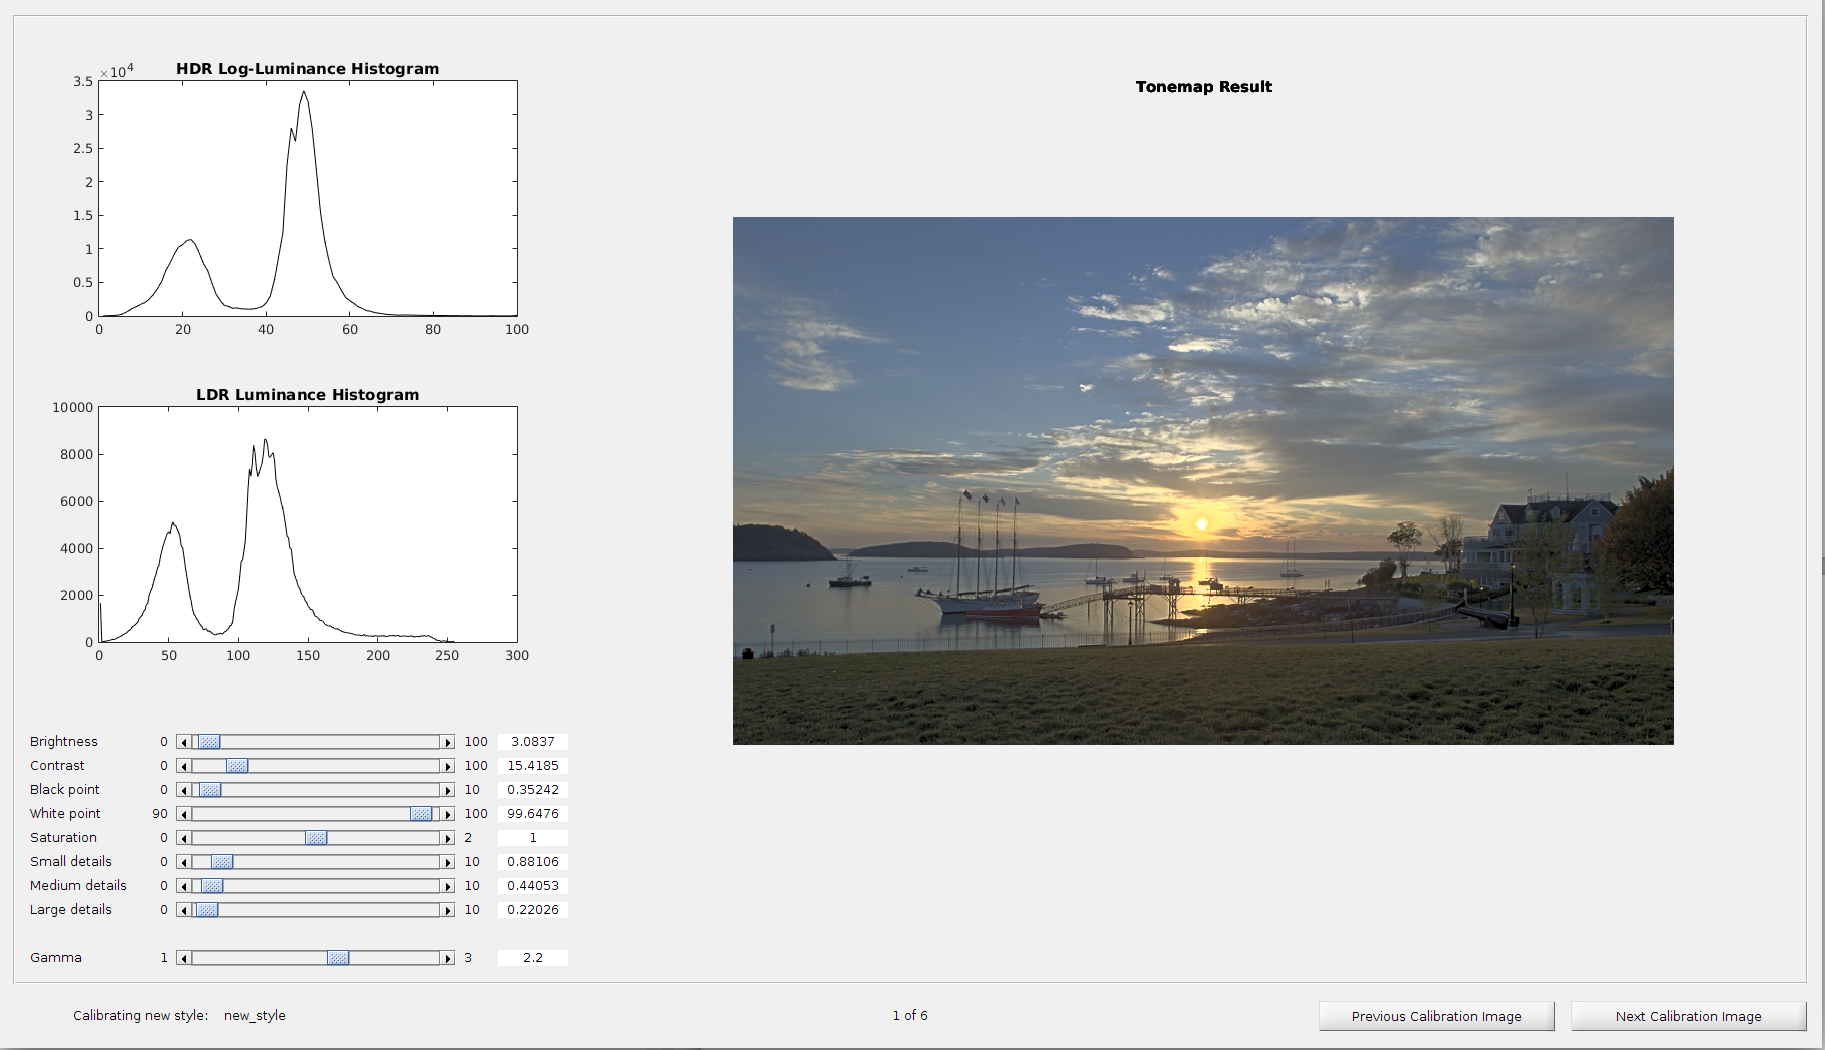
\includegraphics[height=0.85\textwidth]{figures/chapter5/ui_screenshot.png}
\caption{User interface for calibration phase}
\label{fig:calibration_phase}
\end{center}
\end{figure}
\end{landscape}
}

\subsection{Operation}
\label{sec:operation}
In the operation phase, the user selects a style from the preset library that has been created in the calibration phase. Given a new HDR image to be tone mapped with the selected style, the tone mapping parameters \emph{t} (given in Table \ref{tab:tonemap_parameters}) must be determined based on calibration images tone mapping parameters \emph{$t_i$}. In this thesis, this problem is approached as an image similarity problem. If two images are similar according to a similarity metric, their tone mapping parameters should be also similar. After the distances between input image and the calibration images are obtained, the tone mapping parameters are calculated as inverse distance transform~\cite{Shepard1968}:

\begin{equation}
\label{eq:inv_distance_transform}
    \mathbf{t} = {{\sum _{i=1} ^{N} {1 \over {d(\mathbf{f}, \mathbf{f_i})}} \mathbf{t_i}} \over {\sum _{i=1} ^{N} {1 \over {d(\mathbf{f}, \mathbf{f_i})}}}}
\end{equation}

Here, $\mathbf{f}$ is the feature vector of the current input image and $\mathbf{f_i}$ the feature vector for the calibration image $i$ and $\mathbf{t}$ its computed tone mapping parameters. Lastly, the function $d$ calculates the similarity between two feature vectors.

In~\cite{akyuz2013style}, images are represented with HSV histograms~\cite{Ben2006} and histograms of gradients~\cite{dalal2005histograms} to capture colorimetric and structural properties of the images. HDR images varies highly on pixel values and it is hard to compare them directly. To overcome this, images are tone mapped to the interval $[0,1]$:

\begin{equation}
    L_{out} = {{L_{in}} \over {1 + L_{in}}}, 
\end{equation}

and color channels are transformed with:

\begin{equation}
    \mathbf{C_{out}} = {{\mathbf{C_{in}}}\over{L_{in}}} L_{out}.
\end{equation}

The feature vector is then computed using transformed values, as a $60$ dimensional vector, $3x15$ bins for HSV histogram and $15$ bins for gradient histogram. 

Unfortunately, treating histograms as high dimensional points and computing their Euclidean distances does not yield correct results as this ignores the proximity information of the bins. For instance, although the histogram $H1 = (1, 0, 0, \cdots, 0)$ is closer to
$H2 = (0, 1, 0, \cdots, 0)$ than $H3 = (0, 0, 1, \cdots, 0)$, their Euclidean distances are equal. To circumvent this problem, each histogram is convolved with a 1-D Gaussian $(\sigma = 0.7)$ prior to computing their distances ~\cite{Ben2006}. Circular similarity of the hue histogram is also accounted. Thus the final distance metric between two feature vectors \textbf{$f_i$} and \textbf{$f_j$} become:
\begin{equation}
\label{eq:distance_metric}
    d(\mathbf{f_i, f_j}) = \mathbf{(f_i - f_j)}^T\mathbf{(f_i-f_j)},
\end{equation}

where \textbf{$f$} is the combined histogram. This metric is used to measure the similarity between input HDR image and calibration images. Also the same distance metric is used to cluster Fairchild dataset in order to pick calibration images.

After tone mapping parameters are calculated with parameter interpolation, HDR image is tone mapped and presented to the user in a similar user interface like Figure~\ref{fig:calibration_images}. User can do the final adjustments and save the tone mapped LDR image. Figure~\ref{fig:gallery} shows a gallery of the obtained tone mapping results. Note that despite the large variation of the image content, the selected styles are successfully applied to each image.

\begin{figure}
\begin{center}
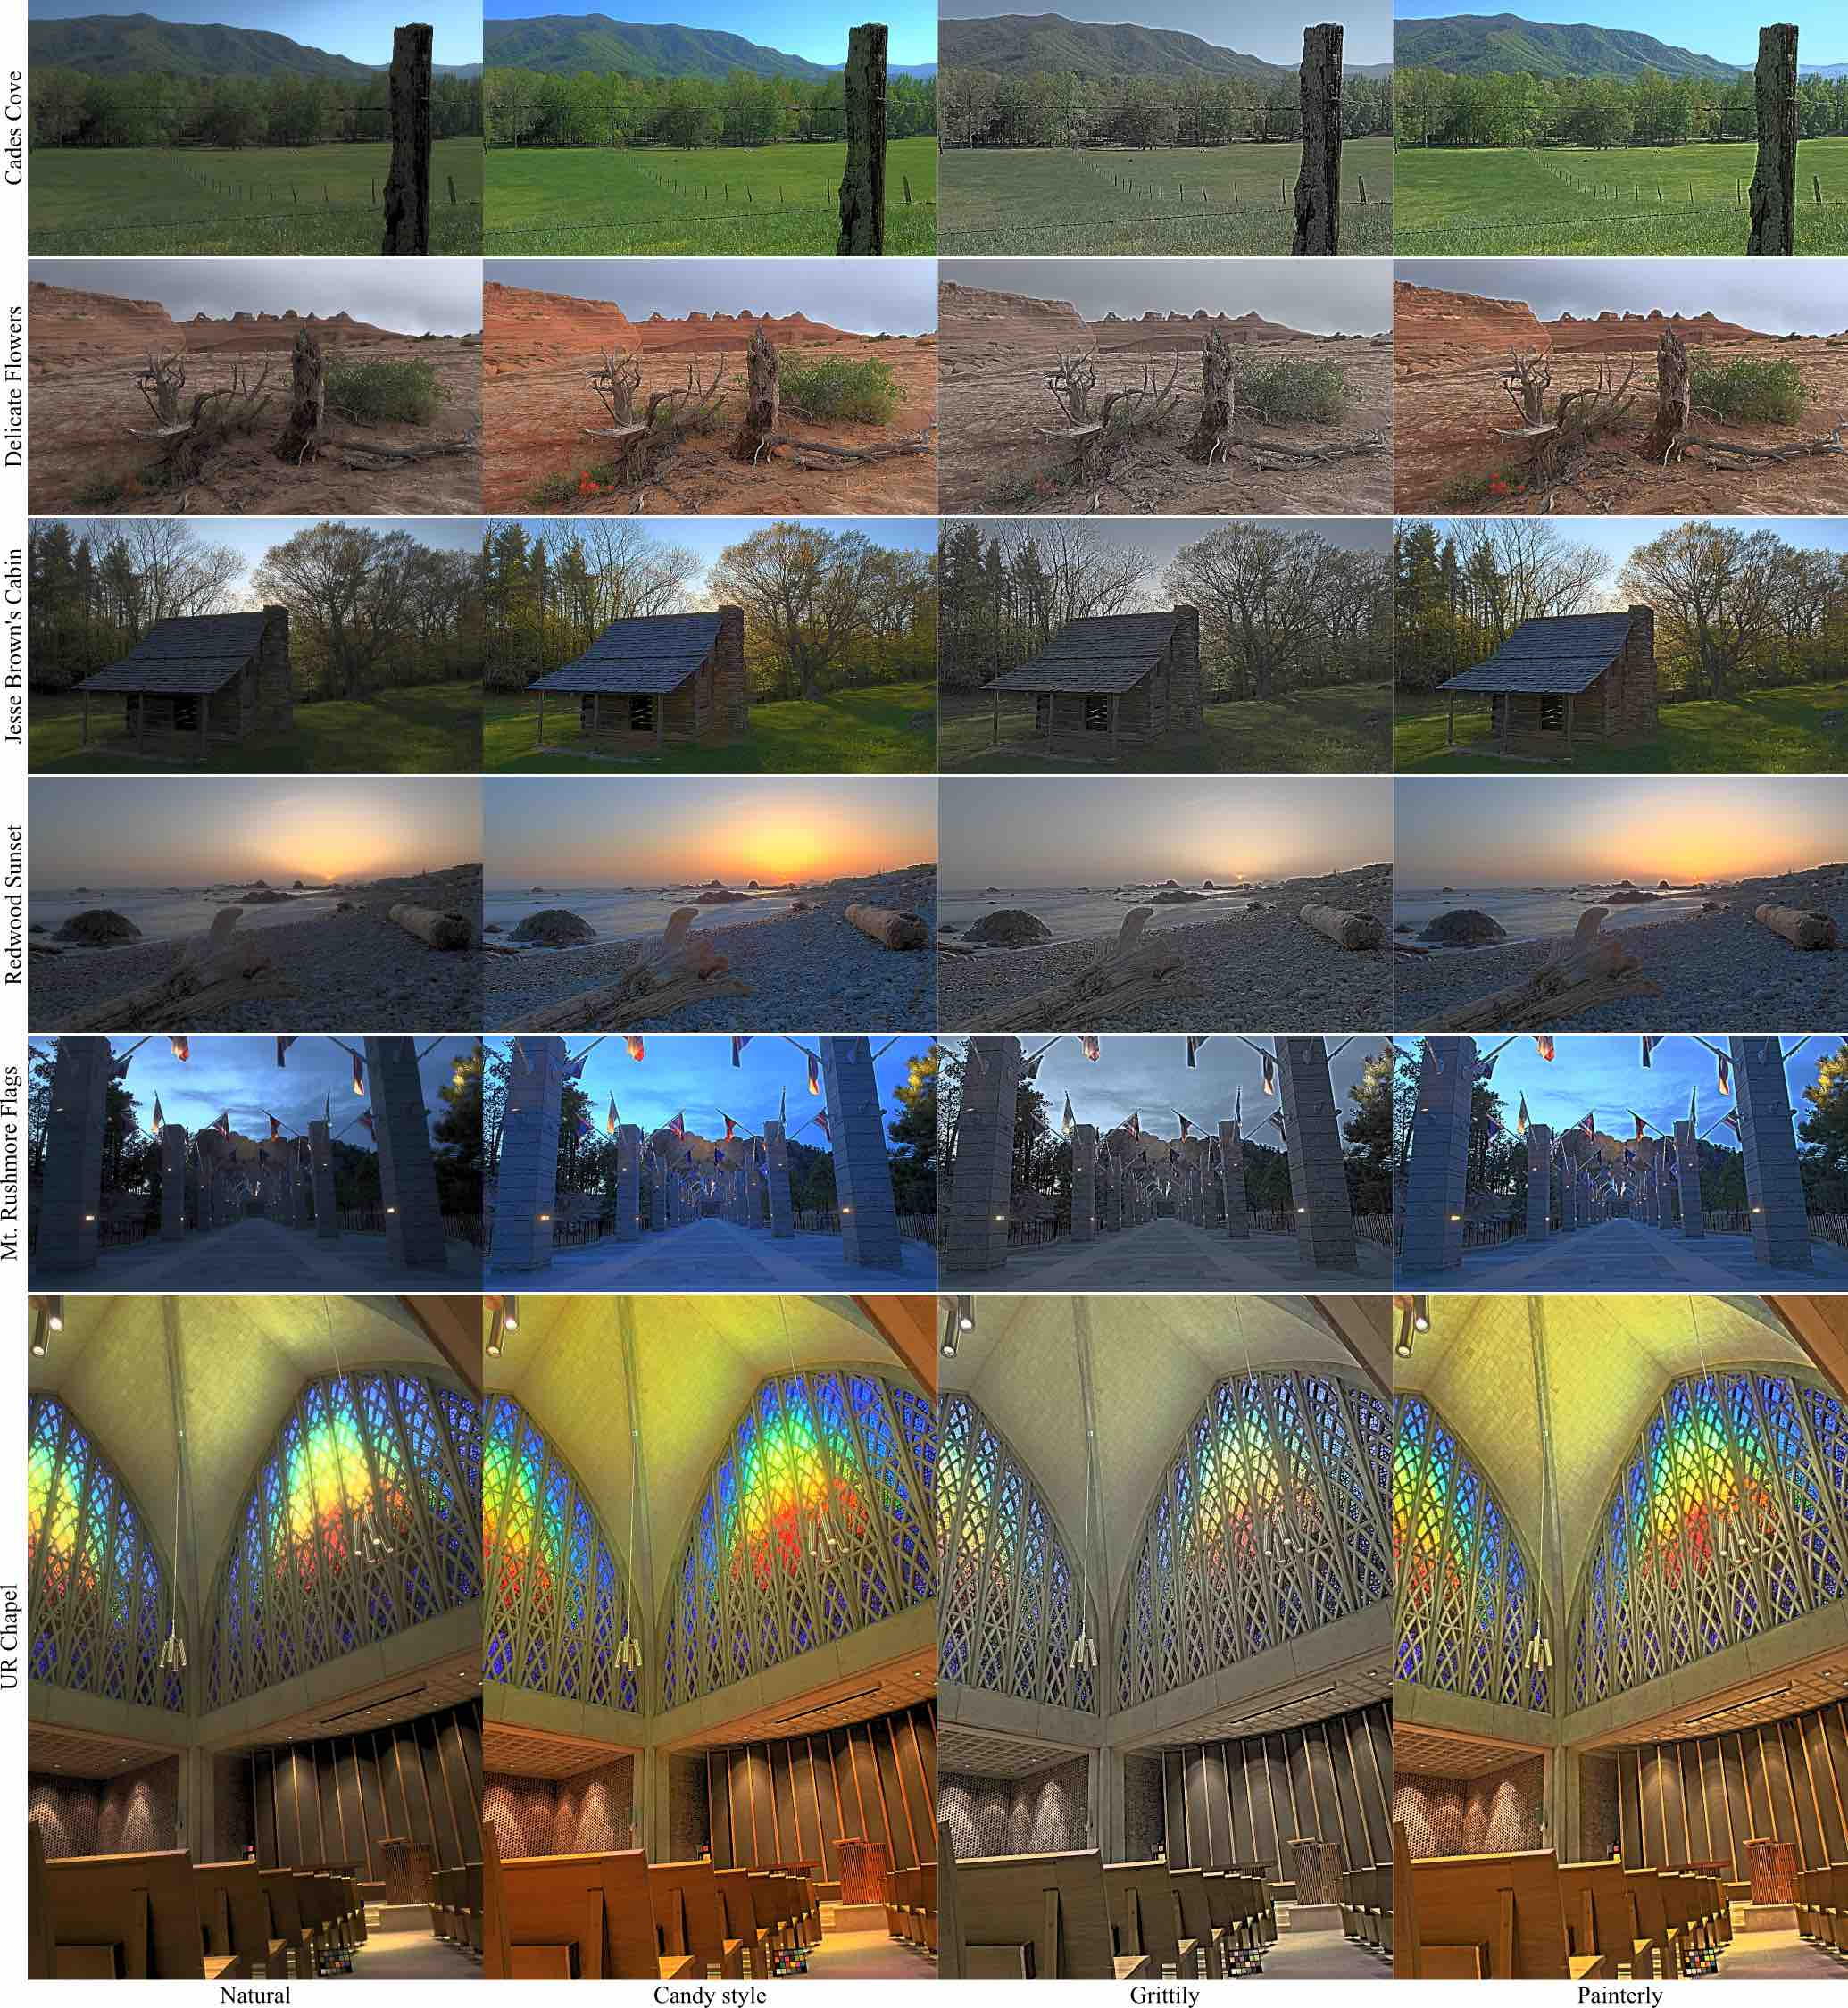
\includegraphics[width=\textwidth]{figures/chapter5/style_based/gallery_small.jpg}
\caption{All of these images are automatically tone mapped using the four styles that are generated.}
\label{fig:gallery}
\end{center}
\end{figure}

To sum up, tone mapping can be an artistic process that would result with different look and feel of the same scene instead of achieving a single "correct" look. The tone mapping methodology given in this chapter is versatile enough to create new styles with a small set of calibration images. And more importantly, with the leverage of image similarity, it is possible to apply the created styles to new HDR images automatically which can have quite different characteristics. However the similarity approach given in this chapter is rather straight forward and there is room for improvement. In the following section, two different similarity models backed up by a user study are suggested to improve style-based tone mapping.

\section{Improvements to Style-based Tone Mapping}
\label{sec:improvements}

Although style based tone mapping has achieved some success for consistently tone mapping different images, the image similarity method given in Section~\ref{sec:operation} can be improved with the findings from the conducted user study. In this section, two modifications of this method that are made possible by the experimental findings of the user study is given. The first technique uses all of the image features utilized in Section~\ref{sec:operation} with different weights to estimate tone mapping parameters in the operation phase. Meanwhile, the second technique relates tone mapping parameters and image features for the estimation.

\subsection{Parameter Interpolation with All Features}
\label{sec:all_features}

In the first modification, the model features given in Table \ref{tab:table_feature} are extracted from the selected HDR image and calibration images. Then, the distances between these features are calculated separately using the corresponding distance metrics given in the same table. After that, the weighted average of these feature distances are calculated. The weights used are the coefficients of the logistic regression model (Equation \ref{eq:log_regression}) obtained from the user experiment, with the idea that less important features should also contribute less to the distance. This operation can be summarized with the following equation:

\begin{equation}
    d_i = \sum_{j=1}^{6}c_j d_j(\mathbf{f_i}, \mathbf{f_{ij}})
\end{equation}

where $c_j$ is the coefficient of the $j^{th}$ feature, $\mathbf{f_j}$ is the $j^{th}$ feature of the input image, $\mathbf{f_{ij}}$ is the same for the $i^{th}$ calibration image, and finally $d_j$ is the distance metric for the $j^{th}$ feature. The result $d_i$ represents the combined distance between the input image and the corresponding calibration image. These combined distances are calculated between the selected HDR image and all calibration images. The tone mapping parameters for the selected HDR image are then interpolated using inverse distance transform as in Equation \ref{eq:inv_distance_transform}. This method differs from the initially presented approach in several aspects: 

\begin{itemize}
    \item Using a different and more representative set of features, luminance which is one of the most important features of HDR images has a separate feature vector,
    \item More suitable distance metrics for feature types, for example, EMD takes into account bin proximity for calculating differences between histograms,
    \item Instead of using a single fused feature vector, each feature distance calculated separately,
    \item Employing a weighted average of feature vector distances with weights obtained from a user experiment, compared to using equal weight.
\end{itemize}

In Figure~\ref{fig:algo_updated}, the modified style-based tone mapping algorithm is shown. Note that while the calibration phase has not changed, the operation phase has been adjusted with the changes listed above compared to the initial version of the algorithm given in Figure~\ref{fig:calibration_operation}. 

\begin{figure}
    \centering
    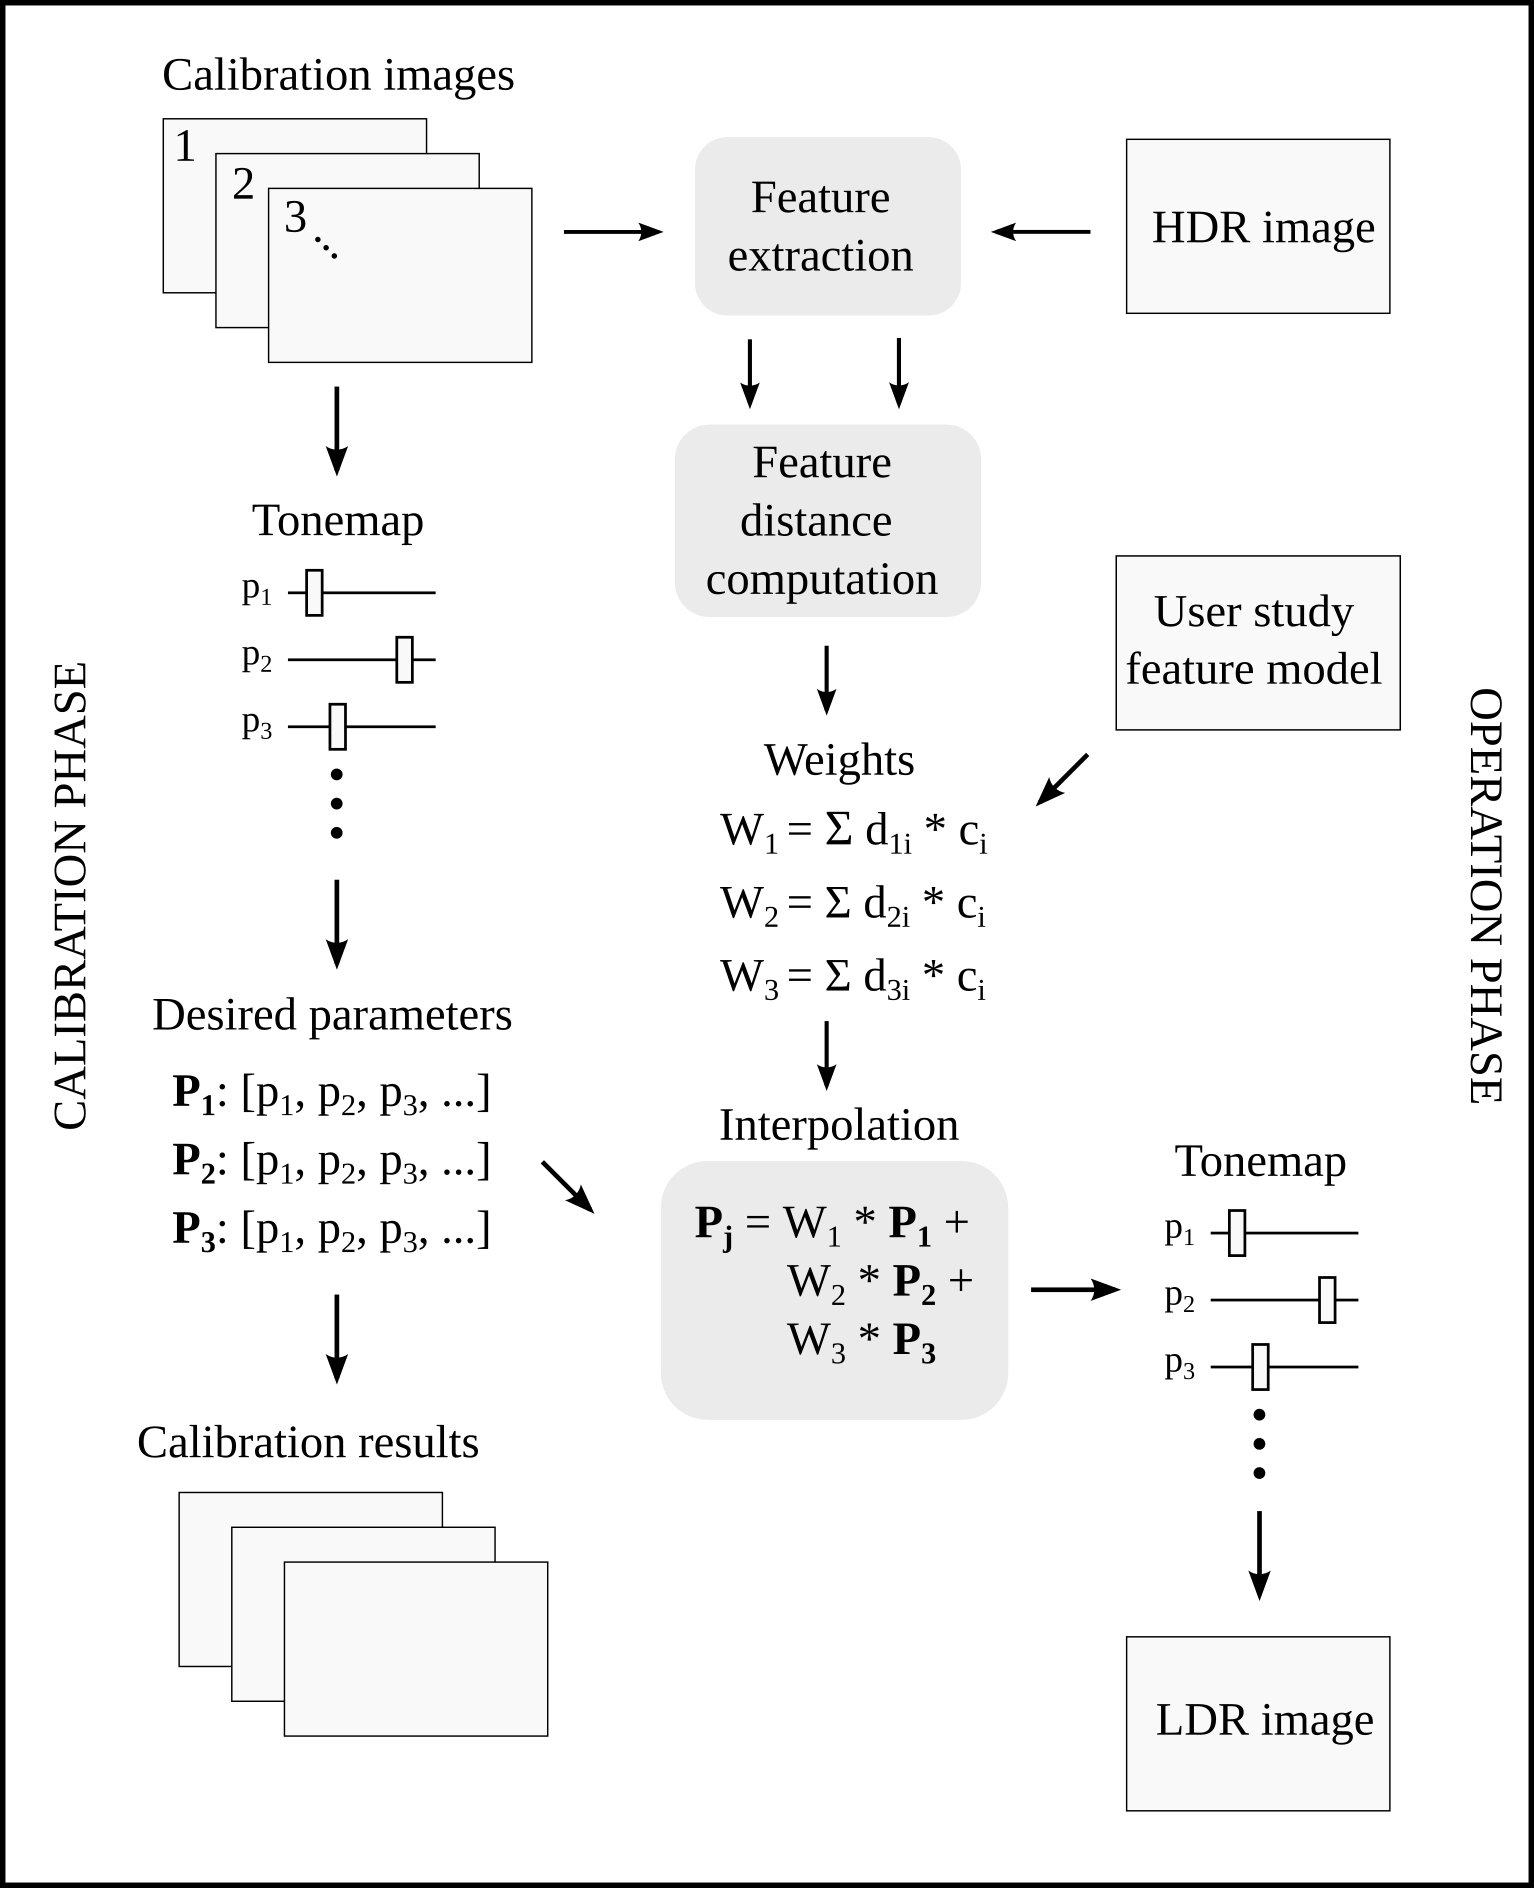
\includegraphics[width=\textwidth]{figures/algorithm_updated.png}
    \caption{Modified style-based tone mapping algorithm with the findings of the user experiment. Compared to the initial method given in Figure~\ref{fig:calibration_operation}, more representative set of features are extracted and distances between these features are computed separately. Besides, instead of using equal weights on feature distances, the weights estimated from user study are employed.}
    \label{fig:algo_updated}
\end{figure}

\subsection{Parameter Interpolation with Related Features}
\label{sec:related_features}
While the previous approach calculates a single distance value between the given image and calibration images and use this value to interpolate all tone mapping parameters, the second modification described in this section relates the model features with the tone mapping parameters and interpolates individual tone mapping parameters with different weights. In order to achieve this, the relationships defined in Table~\ref{tab:feature_mapping} are used.

\begin{table}
\caption{Model features used for interpolation of tone mapping parameters.}
\centering
\begin{tabular}{l | l}
\label{tab:feature_mapping}
\textbf{Tone mapping parameter} & \textbf{Model feature}\\
\hline
Brightness ($t_b$) & Luminance \\
Contrast ($t_c$) & Luminance \\
Black point ($t_{bp}$) & Luminance \\
White point ($t_{wp}$) & Luminance \\
Color saturation ($t_s$) & Color \\
Small detail strength ($t_{\lambda_s}$) & Texture \\
Medium detail strength ($t_{\lambda_m}$ ) & Texture \\
Large detail strength ($t_{\lambda_l}$) & Texture
\end{tabular}
\end{table}


As an example, the brightness parameter $t_b$ is computed by interpolating the $t_{b_i}$ parameters of the calibration images by using the similarity between the luminance features:

\begin{equation}
   t_b = { {\sum_{i=1}^N { {1} \over {d_{lum} (lum, lum_i)} } t_{b_i} } \over {\sum_{i=1}^N} { {1} \over {d_{lum} (lum, lum_i)} } }
\end{equation}

Other tone mapping parameters that are related to the model features are interpolated analogously. Because GIST and deep learning features are not directly linked to a specific appearance phenomenon but are measures of overall similarity between the given images, they are not directly linked to specific tone mapping parameters. Instead these features are experimented with merging them using the individually interpolated parameters as follows: 

\begin{equation}
   \mathbf{t} = w_0\mathbf{t_0} + w_1\mathbf{t_1} + w_2\mathbf{t_2}, 
\end{equation}

where $\mathbf{t_0}$ represents individually interpolated TMO parameters (given in Table~\ref{tab:feature_mapping}), $\mathbf{t_1}$ TMO parameters interpolated as a whole using GIST similarity only, and $\mathbf{t_2}$ TMO parameters interpolated as a whole using solely deep learning feature similarity. The weights control the influence of TMO parameters that are computed by using these different approaches.

\subsection{Results}
In Figure~\ref{FigStyle}, several results are compared that obtained by using the initial style based tone mapping method as well as with the two modifications proposed in the previous sections, Section~\ref{sec:related_features} and Section~\ref{sec:all_features}. 

In the first row of the figure, the tone mapping results of the ``Paul Bunyan'' scene from the HDR Photographic Survey~\cite{fairchild2007hdr} is shown. This scene depicts a bright outdoors environment with colorful foreground objects. It may be noted that all results are similar but the individual parameter interpolation with equally weighted GIST and deep learning features (d) has slightly higher contrast (please refer to Appendix~\ref{app:results} with high resolution images for better comparison). The overall \emph{candy} style is preserved in all images. 

In the second row of the figure, ``Peppermill'' night scene from the same dataset is shown. This is a night scene of a street with some bright lights and banners. For this scene the difference of the second modification, parameter interpolation with related features, is more clear as images in (c) and (d) exhibit a darker rendering, which is more suitable for a night scene. The reason for this darkening effect is that the brightness parameter, $t_b$, for tone mapping becomes more similar to the $t_b$ parameter of the night image in the calibration images due to the similarity of the \emph{luminance} features between these images. The addition of GIST and deep learning features with equal weight in (d) yields a slightly brighter image compared to (c). Similar to the results of the previous image overall \emph{candy} style is preserved also in this image. Appendix~\ref{app:results} has higher resolution versions of the results for more clear observation of the differences.


\afterpage{
\begin{landscape}
\begin{figure}
\begin{subfigure}[b]{0.40\textwidth}
    \centering
    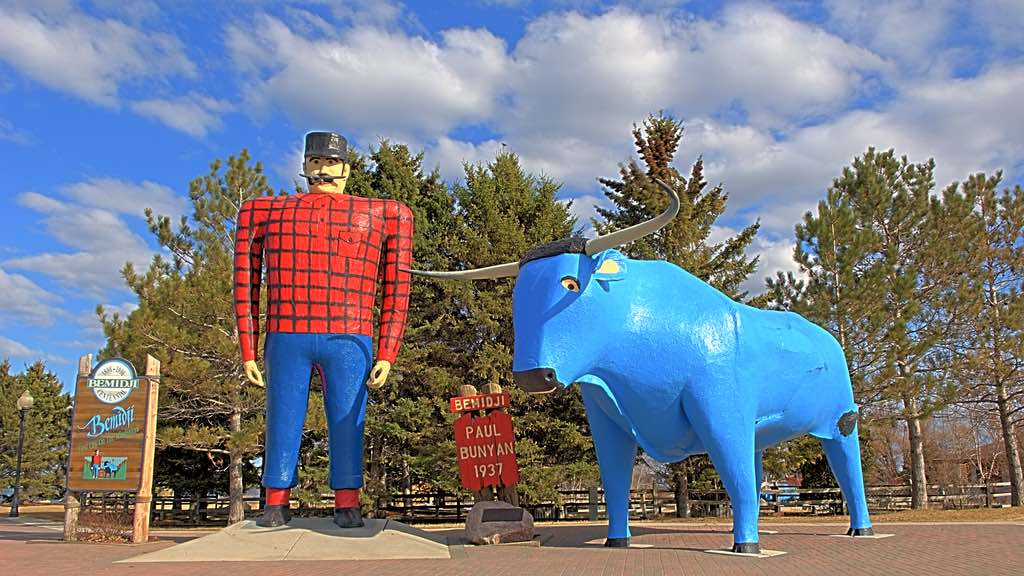
\includegraphics[width=\textwidth]{figures/chapter5/style_based/PaulBunyan_hdrcandy_v1_small.jpg}
    \caption{Initial}
    \label{FigStyle:original_paul_bunyan}
\end{subfigure}\hfill
\begin{subfigure}[b]{0.40\textwidth}
    \centering
    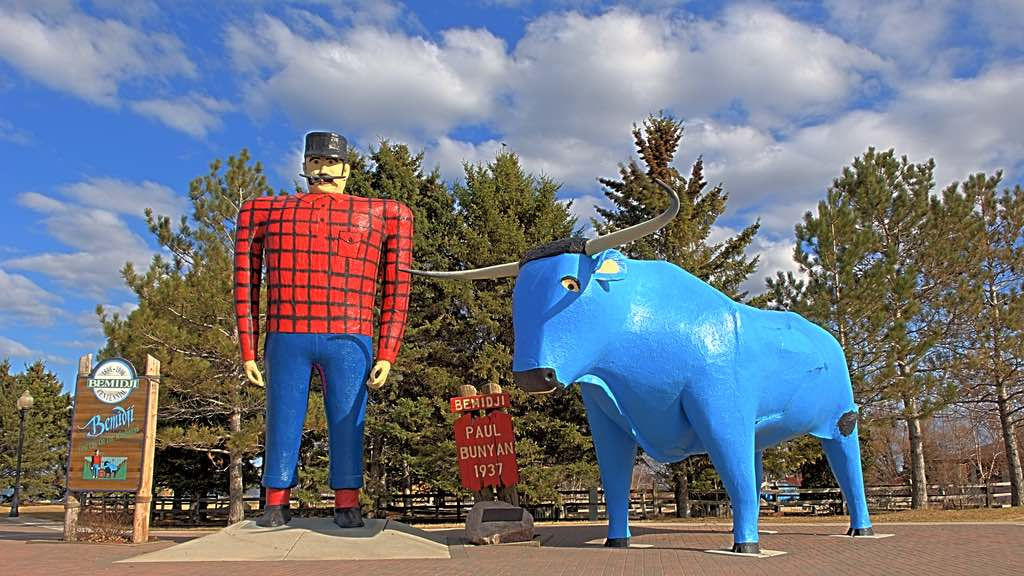
\includegraphics[width=\textwidth]{figures/chapter5/style_based/PaulBunyan_hdrcandy_v2_small.jpg}
    \caption{Version I}
    \label{FigStyle:VerI_paul_bunyan}
\end{subfigure}\hfill
\begin{subfigure}[b]{0.40\textwidth}
    \centering
    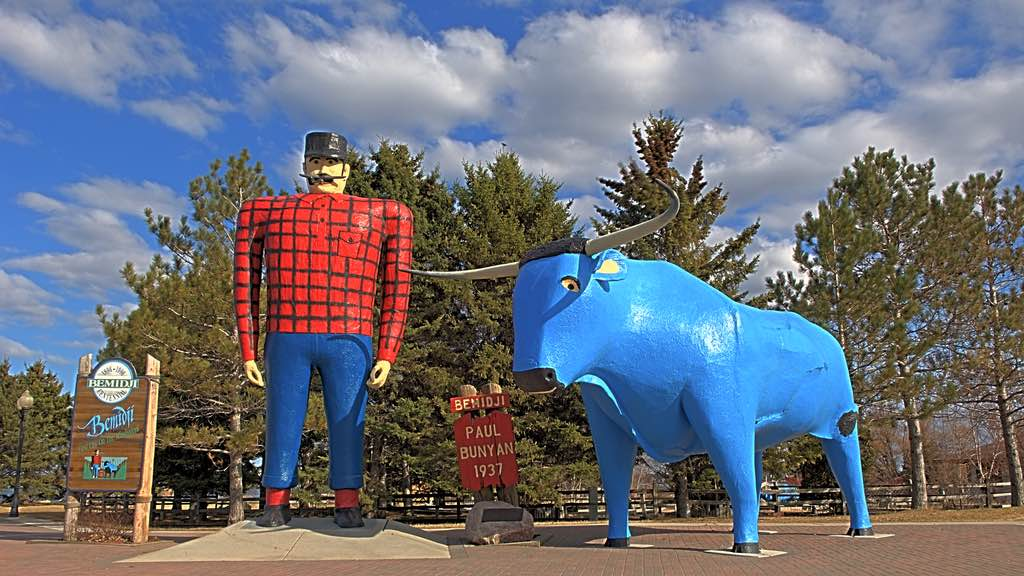
\includegraphics[width=\textwidth]{figures/chapter5/style_based/PaulBunyan_hdrcandy_w0_1_small.jpg}
    \caption{$w_0 = 1$, $w_1 = w_2 = 0$}
    \label{FigStyle:VerIIa_paul_bunyan}
\end{subfigure}\hfill
\begin{subfigure}[b]{0.40\textwidth}
   \centering
    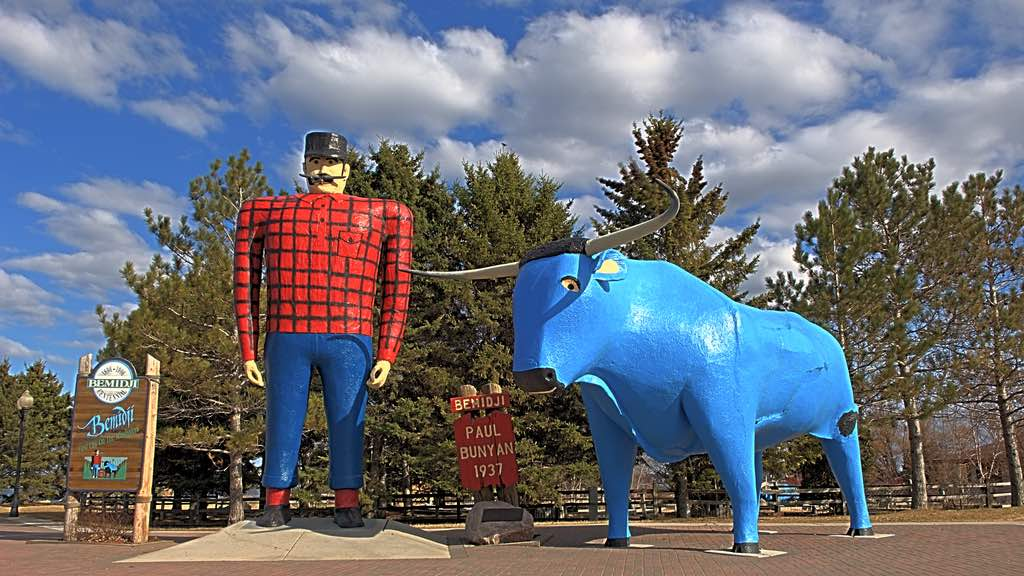
\includegraphics[width=\textwidth]{figures/chapter5/style_based/PaulBunyan_hdrcandy_w0_w1_w2_small.jpg}
    \caption{$w_0 = w_1 = w_2 = \frac{1}{3}$}
    \label{FigStyle:VerIIb_paul_bunyan}
\end{subfigure}\\
\begin{subfigure}[b]{0.40\textwidth}
    \centering
    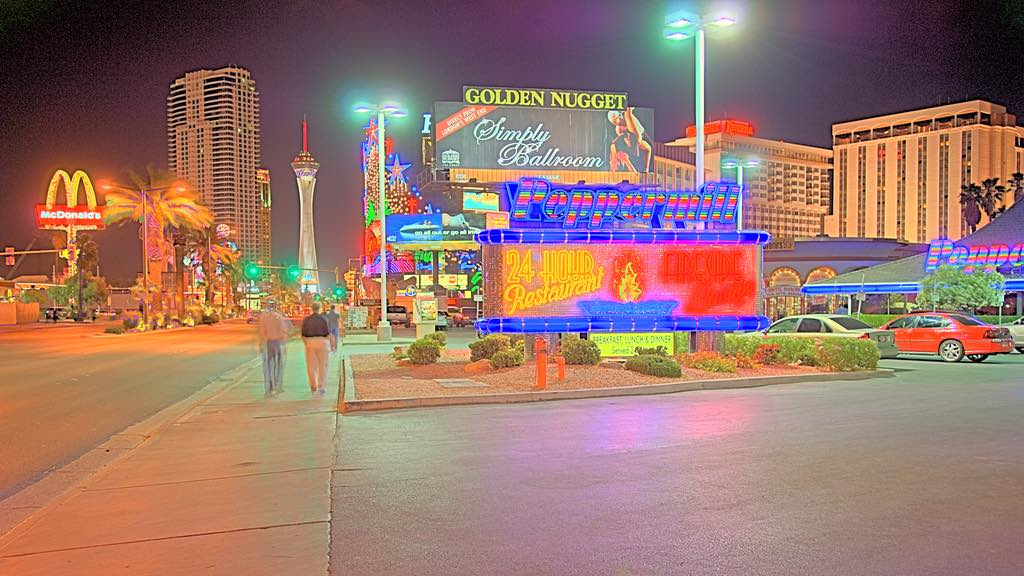
\includegraphics[width=\textwidth]{figures/chapter5/style_based/Peppermill_hdrcandy_v1_small.jpg}
    \caption{Initial}
    \label{FigStyle:original_peppermill}
\end{subfigure}\hfill
\begin{subfigure}[b]{0.40\textwidth}
    \centering
    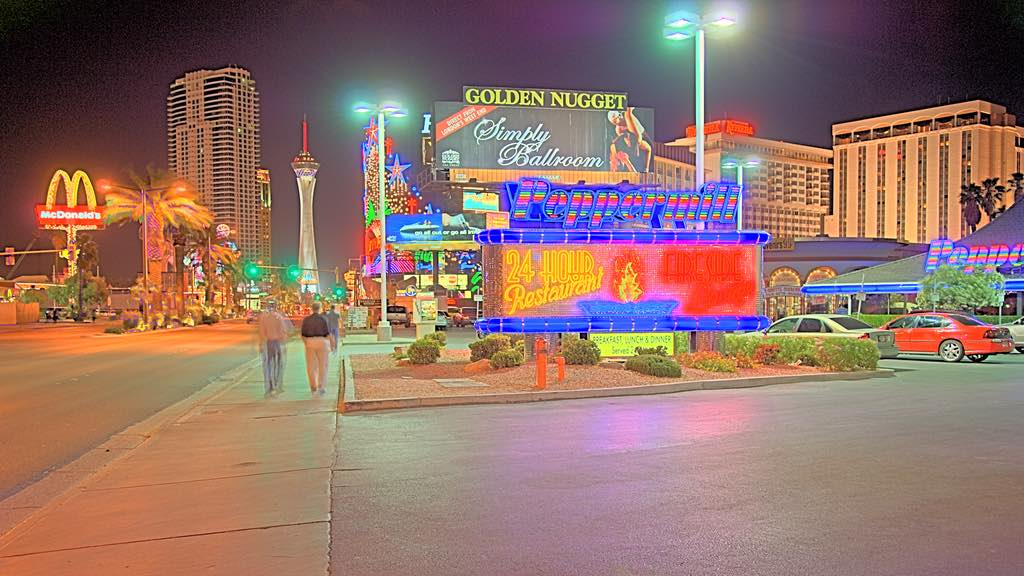
\includegraphics[width=\textwidth]{figures/chapter5/style_based/Peppermill_hdrcandy_v2_small.jpg}
    \caption{Version I}
    \label{FigStyle:VerI_peppermill}
\end{subfigure}\hfill
\begin{subfigure}[b]{0.40\textwidth}
    \centering
    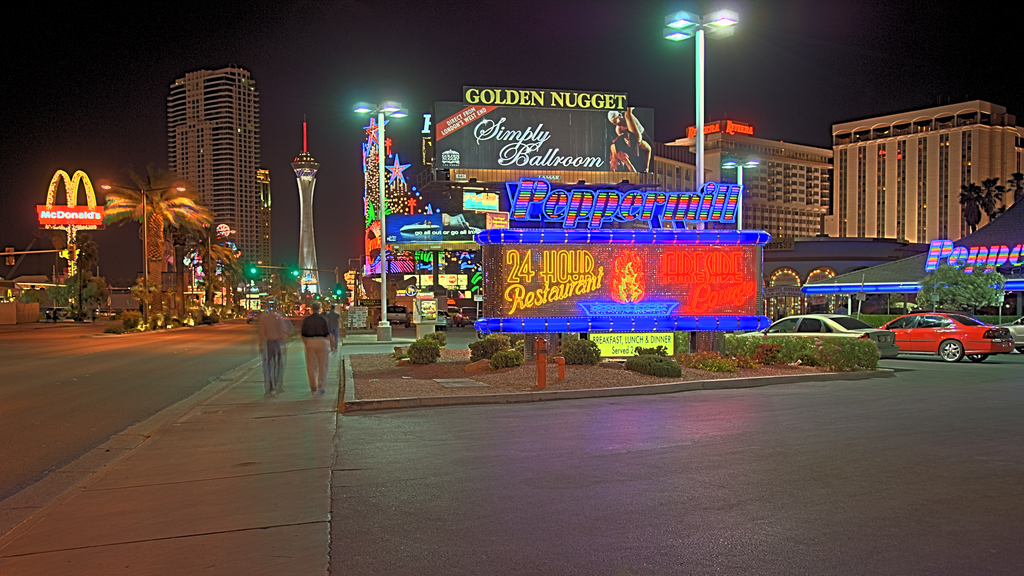
\includegraphics[width=\textwidth]{figures/chapter5/style_based/Peppermill_hdrcandy_w0_1.png}
    \caption{$w_0 = 1$, $w_1 = w_2 = 0$}
   \label{FigStyle:VerIIa_peppermill}
\end{subfigure}\hfill
\begin{subfigure}[b]{0.40\textwidth}
    \centering
    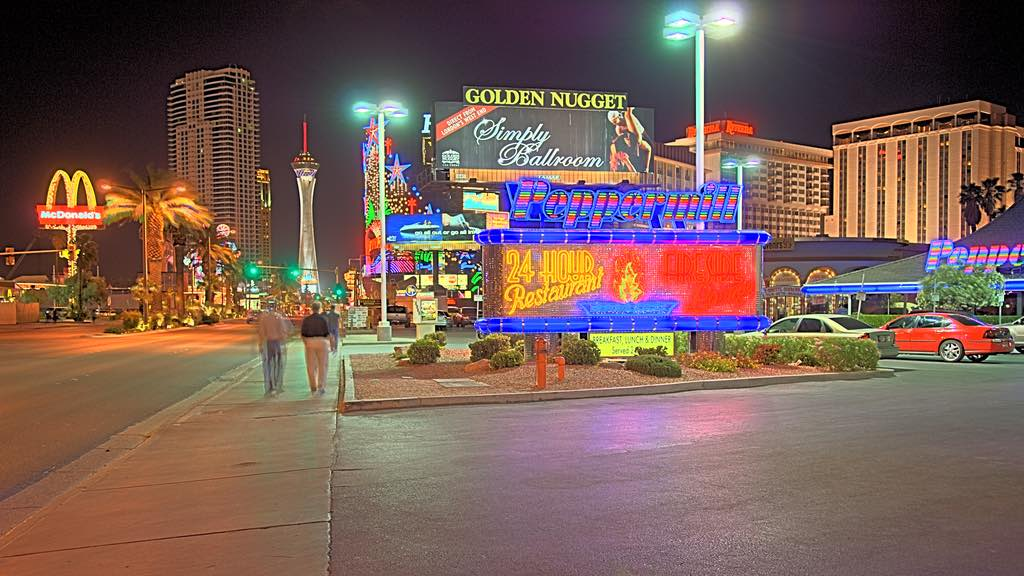
\includegraphics[width=\textwidth]{figures/chapter5/style_based/Peppermill_hdrcandy_w0_w1_w2_small.jpg}
    \caption{$w_0 = w_1 = w_2 = \frac{1}{3}$}
    \label{FigStyle:VerIIb_peppermill}
\end{subfigure}\hfill
\caption{Application of the user study findings for the style-based tone mapping
    problem.  Initial results are shown in the first column, followed
        by Version I in the second column and two variants of Version II
in the last two columns.}
\label{FigStyle}
\end{figure}
\end{landscape}}
